\documentclass[14pt,a4paper,report]{report}
\usepackage[a4paper, mag=1000, left=2.5cm, right=1cm, top=2cm, bottom=2cm, headsep=0.7cm, footskip=1cm]{geometry}
\usepackage[utf8]{inputenc}
\usepackage[english,russian]{babel}
\usepackage{indentfirst}
\usepackage[dvipsnames]{xcolor}
\usepackage[colorlinks]{hyperref}
\usepackage{listings} 
\usepackage{fancyhdr}
\usepackage{caption}
\usepackage{amsmath}
\usepackage{graphicx}
\usepackage{amsmath}
\usepackage{booktabs}
\usepackage{array}
\newcolumntype{P}[1]{>{\centering\arraybackslash}p{#1}}
\hypersetup{
	colorlinks = true,
	linkcolor  = black
}

\usepackage{titlesec}
\titleformat{\chapter}
{\Large\bfseries} % format
{}                % label
{0pt}             % sep
{\huge}           % before-code


\DeclareCaptionFont{white}{\color{white}} 

% Listing description
\usepackage{listings} 
\DeclareCaptionFormat{listing}{\colorbox{gray}{\parbox{\textwidth}{#1#2#3}}}
\captionsetup[lstlisting]{format=listing,labelfont=white,textfont=white}
\lstset{ 
	% Listing settings
	inputencoding = utf8,			
	extendedchars = \true, 
	keepspaces = true, 			  	 % Поддержка кириллицы и пробелов в комментариях
	language = C,            	 	 % Язык программирования (для подсветки)
	basicstyle = \small\sffamily, 	 % Размер и начертание шрифта для подсветки кода
	numbers = left,               	 % Где поставить нумерацию строк (слева\справа)
	numberstyle = \tiny,          	 % Размер шрифта для номеров строк
	stepnumber = 1,               	 % Размер шага между двумя номерами строк
	numbersep = 5pt,              	 % Как далеко отстоят номера строк от подсвечиваемого кода
	backgroundcolor = \color{white}, % Цвет фона подсветки - используем \usepackage{color}
	showspaces = false,           	 % Показывать или нет пробелы специальными отступами
	showstringspaces = false,    	 % Показывать или нет пробелы в строках
	showtabs = false,           	 % Показывать или нет табуляцию в строках
	frame = single,              	 % Рисовать рамку вокруг кода
	tabsize = 2,                  	 % Размер табуляции по умолчанию равен 2 пробелам
	captionpos = t,             	 % Позиция заголовка вверху [t] или внизу [b] 
	breaklines = true,           	 % Автоматически переносить строки (да\нет)
	breakatwhitespace = false,   	 % Переносить строки только если есть пробел
	escapeinside = {\%*}{*)}      	 % Если нужно добавить комментарии в коде
}

\begin{document}

\def\contentsname{Содержание}

% Titlepage
\begin{titlepage}
	\begin{center}
		\textsc{Санкт-Петербургский Политехнический 
			Университет Петра Великого\\[5mm]
			Кафедра компьютерных систем и программных технологий}
		
		\vfill
		
		\textbf{Отчёт по лабораторной работе №2\\[3mm]
			Курс: «Интеллектуальные системы»\\[41mm]
		}
	\end{center}
	
	\hfill
	\begin{minipage}{.4\textwidth}
		Выполнил студент:\\[2mm] 
		Бояркин Н.С.\\
		Группа: 13541/3\\[5mm]
		
		Проверил:\\[2mm] 
		Сазанов А.М.
	\end{minipage}
	\vfill
	\begin{center}
		Санкт-Петербург\\ \the\year\ г.
	\end{center}
\end{titlepage}

% Contents
\tableofcontents
\clearpage

\chapter{Лабораторная работа №2}

\section{Цель работы}

Научиться оформлять отчеты по лабораторным работам.

\section{Программа работы}

\begin{enumerate}
	\item Приведите интенсиональное и экстенсиональные определения двух понятий на ваш выбор.
	\item Постройте ментальную модель знаний в предметной области по вашему выбору с помощью
	интеллект-карт (http://www.mind-map.ru/), которая будет содержать не менее четырех уровней
	ветвления.
	\item Разработайте стратегию принятия решений о приеме на работу кандидата в выбранную Вами
	компанию и записать решение в виде
	\begin{enumerate}
		\item набора продукционных правил (http://itteach.ru/predstavlenie-znaniy/produktsionnaya-model-predstavleniya-znaniy)
		\item дерева принятия решений (http://logic.pdmi.ras.ru/~sergey/teaching/ml/notes-01-dectrees.pdf)
		\item таблицы решений (http://5fan.ru/wievjob.php?id=14722)
	\end{enumerate}
	\item Выделите отличия и сходства следующих моделей представления знаний: алгоритмических,
	логических, сетевых и продукционных и сценарий. Постарайтесь дать объяснения этим различиям.
	\item Что такое онтологии, деревья, фреймы? В чем сходство и различие данных моделей?
	\item Ознакомьтесь с теорией экспертных систем (ЭС). Опишите различие между базой данных (БД) и
	базой знаний (БЗ). Что такое логика предикатов? Что такое «правило вывода»? В чем сильные и
	слабые стороны любой ЭС?
	\item Приведите не менее 3 примеров экспертных систем в каждой из предметных областей,
	разработанную в последнее десятилетие (не позднее 2007), заполнить таблицу.
\end{enumerate}

\clearpage

\section{Ход работы}

\subsection{Задание 1}

\subsubsection{Приведите интенсиональное и экстенсиональные определения двух понятий на ваш выбор.}

Дать «интенсиональное определение» — определить слово или фразу в контексте других слов, как это делается в словаре. Дать «экстенсиональное определение» — указать на пример, как это делают взрослые, когда объясняют что-то ребенку.

\emph{\textbf{Велосипед (интенсиональное)}} -- транспортное средство, приводимое в движение мускульной силой человека через ножные педали или (редко) через ручные рычаги.

\emph{\textbf{Велосипед (экстенсиональное)}} -- транспортное средство, такое как: самокат, машина, гироскутер.

\emph{\textbf{Шкаф (интенсиональное)}} -- род большого стоячего ящика с дверцами для хранения вещей, одежды.

\emph{\textbf{Шкаф (экстенсиональное)}} -- предмет мебели, такой как: стул, кровать, стол.

\subsection{Задание 2}

\subsubsection{Постройте ментальную модель знаний в предметной области по вашему выбору с помощью интеллект-карт}

\begin{figure}[h!]
	\centering
	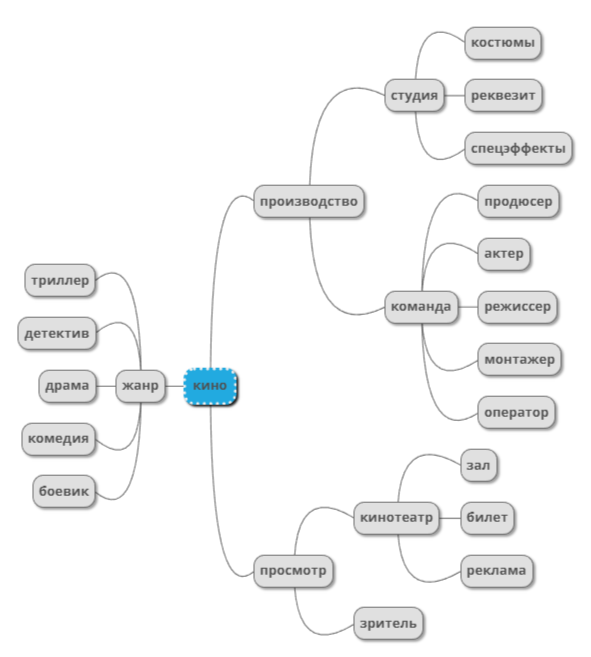
\includegraphics[scale = 0.92]{images/mindmap.png}
	\caption{Ментальная модель знаний}
	\label{image:1}
\end{figure}

\subsection{Задание 3}

Компания: SpaceX

Соискатель: имеет высшее образование, не имеет опыта работы, не знаком с начальником.

Результат выполнения тестового задания: выполнено.

\subsubsection{Стратегия принятия решений о приеме на работу кандидата в виде набора продукционных правил}

П1: Если (соискатель - подходит) то (работа - принять на работу).

П2: Если (соискатель - знакомый начальника) то (соискатель - подходит).

П3: Если (соискатель - решил тестовое задание) и (соискатель - имеет опыт работы) то (соискатель - подходит).

П4: Если (соискатель - решил тестовое задание) и (соискатель - имеет высшее образование) то (соискатель - подходит).\\

\textbf{1-ый проход}

Шаг 1. П1: не работает (не хватает данных (соискатель - подходит)).

Шаг 2. П2: не работает (не хватает данных (соискатель - знакомый начальника)).

Шаг 3. П3: не работает (не хватает данных (соискатель - имеет опыт работы)).

Шаг 4. П4: работает, в базу поступает факт (соискатель - подходит).\\

\textbf{2-ой проход}

Шаг 1. П1: работает, в базу поступает факт (работа - принять на работу).

Шаг 2. П2: не работает (не хватает данных (соискатель - знакомый начальника)).

Шаг 3. П3: не работает (не хватает данных (соискатель - имеет опыт работы)).

Шаг 4. П4: работает, в базу поступает факт (соискатель - подходит).\\

\textbf{Вывод: принять на работу}

\subsubsection{Стратегия принятия решений о приеме на работу кандидата в виде дерева принятия решений}

\begin{figure}[h!]
	\centering
	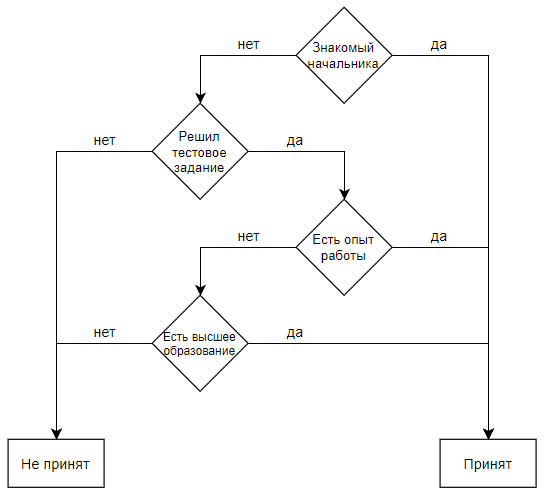
\includegraphics[scale = 0.80]{images/tree.png}
	\caption{Дерево принятия решений}
	\label{image:2}
\end{figure}

\clearpage

\subsubsection{Стратегия принятия решений о приеме на работу кандидата в виде таблицы решений}

\begin{table}[h!]
	\centering
	\bgroup
	\def\arraystretch{1}
	\begin{tabular}{ | P{1.8cm} | P{1.8cm} | P{1.8cm} | P{1.8cm} | P{1.8cm} | }
		\hline
		Знакомый начальника & Решил тестовое задание & Есть опыт работы & Есть высшее образование & Результат 
		\\ \hline
		
		- & - & - & - & - \\ \hline
		
		- & - & - & + & - \\ \hline
		
		- & - & + & - & - \\ \hline
		
		- & - & + & + & - \\ \hline
		
		- & + & - & - & - \\ \hline
		
		- & + & - & + & + \\ \hline
		
		- & + & + & - & + \\ \hline
		
		- & + & + & + & + \\ \hline
		
		+ & - & - & - & + \\ \hline
		
		+ & - & - & + & + \\ \hline
		
		+ & - & + & - & + \\ \hline
		
		+ & - & + & + & + \\ \hline
		
		+ & + & - & - & + \\ \hline
		
		+ & + & - & + & + \\ \hline
		
		+ & + & + & - & + \\ \hline
		
		+ & + & + & + & + \\ \hline
		
	\end{tabular}
	\egroup
	\caption{Таблица решений}
	\label{table:1}
\end{table}

\subsection{Задание 4}

\subsubsection{Выделите отличия и сходства следующих моделей представления знаний: алгоритмических, логических, сетевых и продукционных и сценарий. Постарайтесь дать объяснения этим различиям.}

К \textbf{алгоритмическим моделям} относятся такие, в которых критерии и (или) ограничения описываются математическими конструкциями, включающими логические условия, приводящие к разветвлению вычислительного процесса, и так называемые имитационные модели — моделирующие алгоритмы, имитирующие поведение элементов изучаемого объекта и взаимодействие между ними в процессе функционирования [1]

При построении \textbf{логических моделей} вся информация, необходимая для решения прикладных задач, рассматривается как совокупность фактов и утверждений, которые представляются как формулы в некоторой логике [2]

\textbf{Сетевая модель} отображает взаимосвязи операций и порядок их выполнения. Операции логически упорядочены во времени в том смысле, что одни операции нельзя начать, прежде чем не будут завершены другие. Операция — это работа, для выполнения которой требуются затраты времени и ресурсов [3]

\textbf{Продукционная модель} – это модель, основанная на правилах, позволяющая представить знание в виде предложений типа: «ЕСЛИ условие, ТО действие» [4]

Каждый процесс может быть представлен одной моделью, так и несколькими, в зависимости от удобства использования.

\subsection{Задание 5}

\subsubsection{Что такое онтологии, деревья, фреймы? В чем сходство и различие данных моделей?}

\textbf{Онтология} -- это формальное описание результатов концептуального моделирования предметной области, представленная в форме, воспринимаемой человеком и компьютерной системой [5]

\textbf{Дерево принятия решений} -- дерево, в листьях которого стоят значения целевой функции, а в остальных узлах -- условия перехода, определяющие по какому из ребер идти [6]

\textbf{Фрейм} -- структура данных для представления некоторого концептуального объекта. Информация, относящаяся к фрейму, содержится в составляющих его слотах. Каждый фрейм состоит из произвольного числа слотов, причем несколько из них обычно определяются самой системой для выполнения специфических функций, а остальные определяются пользователем. [7]

Сходство данных моделей состоит в их иерархичности. Для ознакомления со структурой данных лучше использовать фреймы. Однако, для решения прикладных задач удобнее всего использовать деревья принятия решений, так как в них легко прослеживается логика переходов. 

\subsection{Задание 6}

\subsubsection{Ознакомьтесь с теорией экспертных систем (ЭС)}

\textbf{Экспертные системы} это направление исследований в области искусственного интеллекта по созданию вычислительных систем, умеющих принимать решения, схожие с решениями экспертов в заданной предметной области [8]

Экспертные системы имеют одно большое отличие от других систем искусственного интеллекта: они не предназначены для решения каких-то универсальных задач, как например нейронные сети или генетические алгоритмы. Экспертные системы предназначены для качественного решения задач в определенной разработчиками области, в редких случаях – областях [8]

Эксперт предоставляет необходимые знания о тщательно отобранных примерах проблем и путей их решения. Например, при создании экспертной системы диагностики заболеваний врач рассказывает инженеру по знаниям об известных ему заболеваниях. Далее эксперт раскрывает список симптомов, которые сопровождают каждое заболевание и в заключение рассказывает об известных ему методах лечения. Инженер по знаниям, формализует всю полученную информацию в виде базы знаний и помогает программисту в написании экспертной системы [8]

\subsubsection{Опишите различие между базой данных (БД) и базой знаний (БЗ)}

\textbf{База знаний} -- семантическая модель, описывающая предметную область и позволяющая отвечать на такие вопросы из этой предметной области, ответы на которые в явном виде не присутствуют в базе. База знаний является основным компонентом интеллектуальных и экспертных систем [9]

\textbf{База данных} -- совокупность связанных данных, организованных по определенным правилам, предусматривающим общие принципы описания, хранения и манипулирования, независимая от прикладных программ. База данных является информационной моделью предметной области. Обращение к базам данных осуществляется с помощью системы управления базами данных [9]

\subsubsection{Что такое логика предикатов?}

\textbf{Логика предикатов} -– раздел современной логики символической, изучающий рассуждения и другие языковые контексты с учетом внутренней структуры входящих в них простых высказываний, при этом выражения языка трактуются функционально, т.е. как знаки некоторых функций или же знаки аргументов этих функций [10]

\subsubsection{Что такое правило вывода?}

\textbf{Правило вывода} -- если известно, что высказывание «А» влечет (имплицирует) высказывание «В», а также известно, что высказывание «А» истинно, то, следовательно, «В» истинно [11]

\subsubsection{В чем сильные и слабые стороны любой ЭС?}

В настоящее время развитие экспертных систем несколько приостановилось [8], и этому есть ряд причин:

\begin{itemize}
	\item Передача экспертным системам «глубоких» знаний о предметной области является большой проблемой. Как правило, это является следствием сложности формализации эвристических знаний экспертов.
	\item Экспертные системы неспособны предоставить осмысленные объяснения своих рассуждений, как это делает человек. Как правило, экспертные системы всего лишь описывают последовательность шагов, предпринятых в процессе поиска решения.
	\item Отладка и тестирование любой компьютерной программы является достаточно трудоемким делом, но проверять экспертные системы особенно тяжело. Это является серьезной проблемой, поскольку экспертные системы применяются в таких критичных областях, как управление воздушным и железнодорожным движением, системами оружия и в ядерной промышленности.
	\item Экспертные системы неспособны к самообучению. Для того, чтобы поддерживать экспертные системы в актуальном состоянии необходимо постоянное вмешательство в базу знаний инженеров по знаниям. Экспертные системы, лишенные поддержки со стороны разработчиков, быстро теряют свою востребованность.
\end{itemize}

\clearpage

\subsection{Задание 7}

\subsubsection{Приведите не менее 3 примеров экспертных систем в каждой из предметных областей, разработанную в последнее десятилетие (не позднее 2007), заполнить таблицу.}

\begin{table}[h!]
	\centering
	\bgroup
	\def\arraystretch{1}
	\begin{tabular}{ | P{3cm} | P{8cm} | P{2cm} | P{2cm} | }
		\hline
		Предметная область & Название, Страна, Краткое описание & Год & Ссылка 
		\\ \hline
		
		Геология & \textbf{АНАЛОГ} (Россия) -- ищет аналог по любому набору признаков, выбранному в ходе экспертизы, что позволяет пользователю проверять сформулированные им различные гипотезы и сравнивать эффективность различных критериев. & 2009 & [12] \\ \hline
		& \textbf{Астра} (Россия) -- экспертные системы для анализ данных ресурсов и энергопотребления. & 2015 & [13] \\ \hline
		& \textbf{PROSPECTOR} (США) -- действует как консультант, помогающий геологам в поисках залежей руд. Получив данные о геологии района, система оценивает вероятность обнаружить в нем определенные виды минеральных отложений. & 1977 & [14] \\ \hline
		
		Юриспруденция & \textbf{LEXPRO} (Россия) -- экспертная система, позволяющая пользователям получать быстрые ответы, связанные с нормами закона, правовыми отношениями или правовым понятием. & 2007 & [15] \\ \hline
		& \textbf{RiskOver} (Россия) -- позволяет пользователю в интерактивном режиме на профессиональном уровне самостоятельно выявлять юридические риски, возникающие при совершении различного рода сделок. & 2012 & [16] \\ \hline
		& \textbf{Shyster} (США) -- предоставляет консультации в области прецедентного права, которые были указаны юристами-экспертами. Данная юридическая экспертная система реализует простой, прагматичный подход, при котором полезность системы оценивается не в той степени, в которой она имитирует подход адвоката к правовой проблеме, а по качеству ее предсказаний и ее аргументов. & 1993 & [17] \\ \hline
		 
		Медицина & \textbf{Skin Diseases ES} (США) -- онлайн-консультант, консультирующий в области кожных заболеваний. & 2011 & [18] \\ \hline
		& \textbf{Онлайн диагноз} (Россия) -- функционирует по принципу интеллектуального медицинского справочника, указывая врачу возможные варианты диагноза болезней. & 2009 & [19] \\ \hline
		& \textbf{Simptomus} (Россия) -- онлайн-консультант, который проводит диагностику по запросам пользователей & 2011 & [20] \\ \hline
		
		Экономика & \textbf{ТриниДата} (Россия) -- система для помощи в принятии решений для бизнеса и управления предприятием. & 2014 & [21] \\ \hline
		
	\end{tabular}
	\egroup
\end{table}

\clearpage

\begin{table}[h!]
	\centering
	\bgroup
	\def\arraystretch{1}
	\begin{tabular}{ | P{3cm} | P{8cm} | P{2cm} | P{2cm} | }
		\hline
		Предметная область & Название, Страна, Краткое описание & Год & Ссылка 
		\\ \hline

		 & \textbf{Nereid} (Япония) -- данная система была разработана для поддержки принятия решений для оптимизации работы с валютными опционами. Система облегчает дилерскую поддержку для оптимального ответа из возможных представленных вариантов. & 2009 & [22] \\ \hline
		 & \textbf{G2 Expert System} (США) -- автоматизация принятия решений при больших рисках. & 2009 & [23] \\ \hline
		 
		 Биология & \textbf{FaSTR DNA} (США) -- экспертная система для анализа структуры ДНК. & 2008 & [24] \\ \hline
		 & \textbf{CASSIOPE} (США) -- помогает специалистам по структурной химии определять наборы возможных структур неизвестных соединений. & 2009 & [25] \\ \hline
		 & \textbf{Мolgen Five} (Германия) -- экспертная системя для генеалогического тестирования. & 2008 & [26] \\ \hline
		
	\end{tabular}
	\egroup
	\caption{Примеры экспертных систем}
	\label{table:2}
\end{table}

\section{Вывод}

В результате работы я ознакомился понятием экспертных системам, принципом их работы, а также с уже существующими экспертными системами в различных научных дисциплинах. Интерес к данной области сильно упал, что объясняется успехами в области создания действительно интеллектуальных систем: нейронных сетей и роевого интеллекта. Несмотря на это, экспертные системы до сих пор используются для решения множества задач практически во всех областях науки.

\clearpage

\section{Список литературы}

% [20] CONGEN  http://webcache.googleusercontent.com/search?q=cache:iB5Dk50m7CsJ:www.armrobotechs.ru/hp/soft_3.asp%3Fname%3DJUDITH+&cd=1&hl=ru&ct=clnk&gl=ru

% \linebreak

\begin{flushleft}

[1] Алгоритмические модели [Электронный ресурс]. — URL: \href{http://econtool.com/algoritmicheskie-modeli.html}{http://econtool.com/algoritmicheskie-modeli.html} (дата обращения 25.09.2017). \linebreak

[2] Логическая модель знаний [Электронный ресурс]. — URL: \href{http://www.aiportal.ru/articles/knowledge-models/logical-model.html}{http://www.aiportal.ru/articles/knowledge-models/logical-model.html} (дата обращения 25.09.2017). \linebreak

[3] Сетевые модели. Основные понятия и классы сетевых моделей [Электронный ресурс]. — URL: \href{http://bizbook.online/business_menedjment/setevyie-modeli-osnovnyie-ponyatiya-klassyi.html}{http://bizbook.online/business\_menedjment/setevyie-modeli-osnovnyie-ponyatiya-klassyi.html} (дата обращения 25.09.2017).

[4] Продукционная модель знаний [Электронный ресурс]. — URL: \href{http://www.aiportal.ru/articles/knowledge-models/production-model.html}{http://www.aiportal.ru/articles/knowledge-models/production-model.html} (дата обращения 25.09.2017). \linebreak

[5] Онтология [Электронный ресурс]. — URL: \href{http://www.aiportal.ru/articles/other/ontology.html}{http://www.aiportal.ru/articles/other/ontology.html} (дата обращения 25.09.2017). \linebreak

[6] Классификация и регрессия с помощью деревьев принятия решений [Электронный ресурс]. — URL: \href{https://habrahabr.ru/post/116385/}{https://habrahabr.ru/post/116385/} (дата обращения 25.09.2017). \linebreak

[7] Фреймовая модель знаний [Электронный ресурс]. — URL: \href{www.aiportal.ru/articles/knowledge-models/frame-model.html}{www.aiportal.ru/articles/knowledge-models/frame-model.html} (дата обращения 25.09.2017). \linebreak

[8] Экспертные системы [Электронный ресурс]. — URL: \href{http://www.aiportal.ru/articles/expert-systems/expert-systems.html}{http://www.aiportal.ru/articles/expert-systems/expert-systems.html} (дата обращения 25.09.2017). \linebreak

[9] Базы данных и базы знаний.Определения.Отличия.Основные свойства. [Электронный ресурс]. — URL: \href{https://sites.google.com/site/bazydannyhibazyznanij2013/home/bazy-dannyh-i-bazy-znanij-opredelenia-otlicia-osnovnye-svojstva}{https://sites.google.com/site/bazydannyhibazyznanij2013/home/bazy-dannyh-i-bazy-znanij-opredelenia-otlicia-osnovnye-svojstva} (дата обращения 25.09.2017). \linebreak

[10] ЛОГИКА ПРЕДИКАТОВ [Электронный ресурс]. — URL: \href{https://iphlib.ru/greenstone3/library/collection/newphilenc/document/HASHb46c37179b4005520488b4}{https://iphlib.ru/greenstone3/library/collection/newphilenc/document/HASHb46c37179b4005520488b4} (дата обращения 25.09.2017). \linebreak

[11] Правила вывода [Электронный ресурс]. — URL: \href{http://www.aiportal.ru/articles/knowledge-models/modus-ponens.html}{http://www.aiportal.ru/articles/knowledge-models/modus-ponens.html} (дата обращения 25.09.2017). \linebreak

[12] ТЕОРЕТИЧЕСКИЕ ОСНОВЫ РАЗРАБОТКИ ГИБРИДНЫХ ЭКСПЕРТНЫХ СИСТЕМ ДЛЯ ПРОГНОЗА И ОЦЕНКИ РУДНЫХ МЕСТОРОЖДЕНИЙ [Электронный ресурс] . — URL: \href{http://oldvak.ed.gov.ru/common/img/uploaded/files/vak/2010/announcements/Geolog-miner/02-08/CHizhovaIA.pdf}{http://oldvak.ed.gov.ru/common/img/uploaded/files/vak/2010/announcements/Geolog-miner/02-08/CHizhovaIA.pdf} (дата обращения 07.10.2017). \linebreak

[13] Системы контроля и учета тепла, воды, газа, электричества [Электронный ресурс]. — URL: \href{www.astraeng.ru/products.php}{www.astraeng.ru/products.php} (дата обращения 07.10.2017).  \linebreak

[14] Home\&Pro Robotics - экспертные системы. Система PROSPECTOR [Электронный ресурс]. — URL: \href{http://webcache.googleusercontent.com/search?q=cache:kXqAMNaW0HkJ:www.arm-robotechs.ru/hp/soft\_3.asp\%3Fname\%3DPROSPECTOR+\&cd=10\&hl=ru\&ct=clnk\&gl=ru}{http://webcache.googleusercontent.com/search?q=cache:kXqAMNaW0HkJ:www.arm-robotechs.ru/hp/soft\_3.asp\%3Fname\%3DPROSPECTOR+\&cd=10\&hl=ru\&ct=clnk\&gl=ru} (дата обращения 25.09.2017). \linebreak

[15] LEXPRO - экспертная юридическая система [Электронный ресурс]. — URL: \href{http://www.lexpro.ru/}{http://www.lexpro.ru/} (дата обращения 07.10.2017).  \linebreak

[16] RiskOver.ru - экспертная юридическая система [Электронный ресурс]. — URL: \href{http://riskover.ru/}{http://riskover.ru/} (дата обращения 07.10.2017). \linebreak

[17] ИСТОРИЯ ЮРИДИЧЕСКИХ ЭКСПЕРТНЫХ СИСТЕМ [Электронный ресурс]. — URL: \href{http://libraryno.ru/8-1-istoriya-yuridicheskih-ekspertnyh-sistem-2015_inform_tehbologii/}{http://libraryno.ru/8-1-istoriya-yuridicheskih-ekspertnyh-sistem-2015\_inform\_tehbologii/} (дата обращения 07.10.2017). \linebreak

[18] Diagnosis of Skin Diseases using Online Expert System [Электронный ресурс]. — URL: \href{https://www.researchgate.net/publication/215565885_Diagnosis_of_Skin_Diseases_using_Online_Expert_System}{https://www.researchgate.net/publication/215565885\_Diagnosis\_of\_Skin\_Diseases\_using\_Online\_Expert\_System} (дата обращения 07.10.2017). \linebreak

[19] Диагноз-онлайн - информационно-справочный портал о медицине, здоровье и красоте [Электронный ресурс]. — URL: \href{http://diagnos-online.ru/}{http://diagnos-online.ru/} (дата обращения 07.10.2017). \linebreak

[20] Онлайн диагностика заболеваний по симптомам [Электронный ресурс]. — URL: \href{http://simptomus.ru/}{http://simptomus.ru/} (дата обращения 07.10.2017). \linebreak

[21] ТриниДата: управление знаниями, интеграция, мастер-данные, аналитика [Электронный ресурс]. — URL: \href{http://trinidata.ru/}{http://trinidata.ru//} (дата обращения 07.10.2017). \linebreak

[22] Примеры Экспертных систем [Электронный ресурс]. — URL: \href{http://tpl-it.wikispaces.com/\%D0\%9F\%D1\%80\%D0\%B8\%D0\%BC\%D0\%B5\%D1\%80\%D1\%8B+\%D0\%AD\%D0\%BA\%D1\%81\%D0\%BF\%D0\%B5\%D1\%80\%D1\%82\%D0\%BD\%D1\%8B\%D1\%85+\%D1\%81\%D0\%B8\%D1\%81\%D1\%82\%D0\%B5\%D0\%BC}{http://tpl-it.wikispaces.com/Примеры+Экспертных+систем} (дата обращения 07.10.2017). \linebreak

[23] G2 Standard | Gensym [Электронный ресурс]. — URL: \href{http://www.gensym.com/platforms/g2-standard/}{http://www.gensym.com/platforms/g2-standard/} (дата обращения 07.10.2017). \linebreak

[24] Activity of some antiseptics against urinary tract pathogens growing as biofilms on silicone surface [Электронный ресурс]. — URL: \href{https://www.ncbi.nlm.nih.gov/pubmed/19083817}{https://www.ncbi.nlm.nih.gov/pubmed/19083817} (дата обращения 07.10.2017). \linebreak

[25] Knowledge Based Expert Systems in Bioinformatics [Электронный ресурс]. — URL: \href{https://www.intechopen.com/books/expert-systems/knowledge-based-expert-systems-in-bioinformatics}{https://www.intechopen.com/books/expert-systems/knowledge-based-expert-systems-in-bioinformatics} (дата обращения 07.10.2017). \linebreak

[26] MOLGEN [Электронный ресурс]. — URL: \href{http://molgen.de/}{http://molgen.de/} (дата обращения 07.10.2017). \linebreak


\end{flushleft}
	


\end{document}